\label {fs-acker-intro}

% Distributed stream processing engines (SPEs), such as Flink~\cite{carbone2015apache}, Heron~\cite{Kulkarni:2015:THS:2723372.2742788}, or MillWheel~\cite{Akidau:2013:MFS:2536222.2536229}, aim to handle potentially unbounded sequences of data elements. These systems receive input data elements one-by-one, process them, update the internal state, and eventually release results. 

The processing of a data stream without insights on properties of its data elements can be challenging. For example, it may be unclear when a system can prune outdated keyed state~\cite{Tucker:2003:EPS:776752.776780}, release windowed aggregations~\cite{Begoli:2019:OSR:3299869.3314040}, or create a state snapshot for an epoch~\cite{Carbone:2017:SMA:3137765.3137777}.

Each of these scenarios can be considered as a special case of {\em substream management problem}. This problem is to monitor substreams emergence and termination. More formally, a substream is a part of the stream such that all its elements satisfy some predicate. For example, in the case of state pruning, the predicate is {\em [a data element has a key $K$]}, for time window aggregations, the predicate is {\em [a data element is generated with timestamp less than $T$]}, and for state snapshotting it is {\em [a data element belongs to the epoch $E$]}.


% The processing of unbounded data sequences is challenging. The volume of the system state may become unlimited, and SPE needs to optimize state access policy to balance memory consumption and latency of requests. To solve these and many other challenges of stream processing, infinite streams are often split into finite {\em substreams}, that are assumed isolated from each other. This trick allows us to convert a single task on an infinite stream of messages to a stream of tasks on a limited number of messages.

% \noindent {\bf State pruning}. Most SPEs group state by keys that are also used for data partitioning. For example, the task is to aggregate news into stories assigning every news item a story tag. In this case, a story tag will be the key; the properties of the story that are needed for tagging procedure will be the state. The number of stories is not limited, and to prevent overflow~\cite{Tucker:2003:EPS:776752.776780}, SPE can remove state for outdated keys, e.g., for completed stories. In this case, we can consider the stream as a mixture of substreams: one per story.  

% \noindent {\bf Windowed aggregations}. One way to adapt a relational query to a streaming environment is to run it on a window of data elements. This way, an initial stream will be converted into a stream of query results for each window instance. This method is widely applied in online analytics~\cite{traub2018scotty} and is used for streaming SQL implementation~\cite{Begoli:2019:OSR:3299869.3314040}. The window definition, in this case, forms a substream. For example, a sliding window will define a substream for each message in the initial stream.

% \noindent {\bf State snapshotting}. Epoch-based state snapshotting is a popular recovery technique applied in Flink~\cite{Carbone:2017:SMA:3137765.3137777}, Storm~\cite{Toshniwal:2014:STO:2588555.2595641}, Samza~\cite{Noghabi:2017:SSS:3137765.3137770}, IBM Streams~\cite{jacques2016consistent}. This method divides a stream into a sequence of data element chunks called ({\em epochs}). An SPE takes a state snapshot when a regular epoch is {\em atomically} processed. In case of failures, SPE can consistently recover the state from the snapshot~\cite{2015arXiv150608603C}. 

% Each of these scenarios can be considered as a special case of {\em substream management problem}. This problem is to monitor substreams emergence and termination. More formally, a substream is a part of the stream such that all its elements satisfy some predicate. For example, in the case of state pruning, the predicate is {\em [a news item is tagged by story $X$]}, while for time window aggregations, the predicate is {\em [a data element is generated with timestamp less than $T$]}. 

In this paper, we focus only on two signals: substream start and its termination. Tracking a start of a substream is a straightforward task: the first event of a substream will naturally trigger its start. On the contrary, generating a substream termination event is a challenging task, and various properties may be required by practical problems:
\begin{itemize}
    \item Deterministic windowed join requires an order of termination signals to respect the order of input elements (termination events from data producers)~\cite{najdataei2019stretch, gulisano2016scalejoin}.
    \item An epoch is a substream that an SPE should process atomically. A termination event for an epoch should arrive before any elements of the next epoch~\cite{2015arXiv150608603C}.
    \item State pruning problem does not require any specific properties from termination events. However, late termination event receiving may cause sub-optimal memory utilization.
\end{itemize}

% As we can see, the substream management problem appears in many practical scenarios that impose requirements on the termination events. We formalize the substream management problem and generalize its properties. The formalization allows us to verify that a certain solution of the problem is suitable for the mentioned scenarios as well as for the more general problems that require substream management.

A popular substream management method is the punctuations framework~\cite{tucker2003exploiting}. The main idea behind this framework is to divide the stream injecting special elements called {\em punctuations} that define substreams ``borders''. While the punctuations approach is robust and easy-to-implement, it has two limitations:
\begin{enumerate}
    \item The lack of cyclic dataflows support~\cite{carbone2018scalable}. Many real-life applications, including machine learning~\cite{webirte} or graphs processing pipelines~\cite{xu2018fault}, require cyclic dataflows. The absence of a common substream management mechanism for this scenario reduces the applicability of SPEs for such tasks.
    \item High network traffic overhead. Punctuations framework has been initially designed for centralized stream processing~\cite{Tucker:2003:EPS:776752.776780} and requires frequent broadcasts between SPE nodes in distributed implementation. It can influence the end-to-end performance~\cite{DBLP:journals/pvldb/BegoliACHKKMS21} of SPEs and reduce their scalability because present-day deploys can consist of over 1000 nodes~\cite{Carbone:2017:SMA:3137765.3137777}. 
\end{enumerate}
% First, it does not support general cyclic dataflows~\cite{carbone2018scalable}. Second, the ``border'' elements are frequently broadcasted between SPE nodes, so punctuations have high network traffic overhead and can reduce the throughput of an SPE in case of numerous substreams~\cite{Li:2008:OPN:1453856.1453890}. 

\begin{figure}[t]
  \centering
  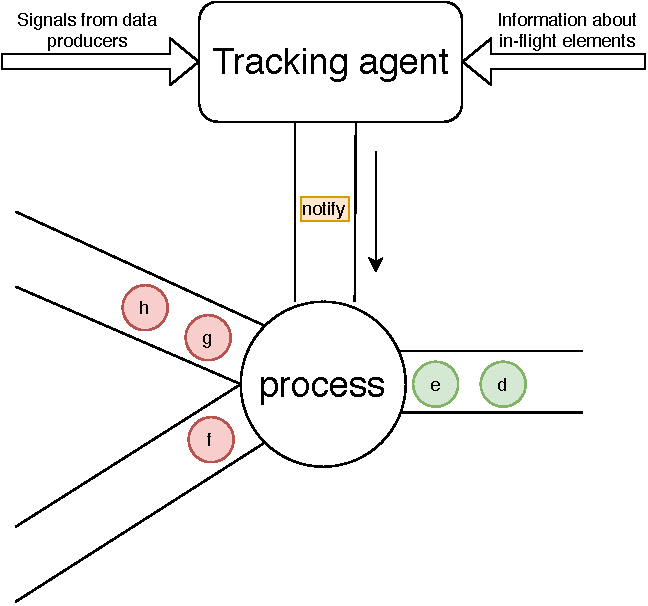
\includegraphics[width=0.20\textwidth]{pics/tracker-scheme.pdf}
  \caption{\tracker\ framework: tracking agent aggregates information about substreams and produces NEOSS}
  \label{tracker_scheme}
\end{figure}

In this work we formalize the substream management problem and show that the network traffic overhead of the punctuations framework is far from the optimal. We also formally define properties of a substream management technique required by various problems such as state snapshotting to ensure that a newly proposed method satisfy them. 

We introduce a new substream management framework called \tracker. The high-level scheme of our method is shown in Figure~\ref{tracker_scheme}. Within this framework, we use a dedicated agent that receives information about substreams from the entire SPE and sends back {\em end-of-substream notifications} (NEOSS). NEOSS messages is propagated through this agent without broadcasting between processes, reducing the amount of extra traffic. Such propagation method is suitable for cyclic dataflows because there is no need to forward service traffic through the cycles.

Basic comparison between the \tracker\ framework and its alternatives is shown in Table~\ref{solutions-overview-table}. Regarding network traffic, $|\Pi|$ is the number of computational nodes and $K$ is the number of substreams. We can outline that the punctuations framework is the only substream management mechanism that supports arbitrary predicates for substreams, so we use it as a baseline approach in the experiments. The commonalities and differences between the \tracker\ framework and alternative solutions are detailed in Section~\ref{fs-acker-related}.

\begin{table}[t]
    \caption{An overview of substream management techniques}
    \label{solutions-overview-table}
    \begin{threeparttable}
        \centering
        \begin{tabular}{|>{\bfseries}c|c|c|c|c|c|} 
          \hline
          Method & Arbitrary predicates & Cycles & Traffic  \\ \hline \hline
          Punctuations & + & - & $O(K|\Pi|^2)$ \\ \hline
          MillWheel* & - & N/A & N/A \\ \hline
          Naiad* & - & + & $O(K|\Pi|^2)$ \\ \hline
          Acker & - & + & $O(K|\Pi|)$ \\ \hline
          \tracker\ & + & + & $O(K|\Pi|)$ \\ \hline
        \end{tabular}
        *progress tracker
    \end{threeparttable}
\end{table}

% A distributed version of the agent allows a system to scale and stay fault-tolerant.

% By tackling challenges, \tracker\ opens an ability to apply substreams-based techniques for new tasks, such as iterative stream processing and new setups, e.g., very granular substreams. We compare the performance of \tracker\ to the punctuations framework applied in most state-of-the-art SPEs. We demonstrate that \tracker\ can outperform punctuations on synthetic and real-world dataflows. We also show a novel application of substream management for a real-world cyclic dataflow. 

In summary, our contributions are as follows:
\begin{enumerate}
    \item We provide a formal model of substream management. This model allows us to compare the properties of various substream management systems.
    \item We present a novel substream management technique that achieves a lower bound of network traffic overhead.
    \item We demonstrate \tracker\ performance in comparison to a state-of-the-art approach on diverse workloads.
\end{enumerate}

The rest of the paper is organized as follows: Section~\ref{fs-acker-preliminaries} formalizes the substream management problem and indicates its main properties. In Section~\ref{fs-acker-tracker}, we introduce a general design of the \tracker\ framework and demonstrate the properties of this substream management solution. Section~\ref{fs-acker-impl} summarizes the implementation of \tracker\. In Section~\ref{fs-experiments}, we show that the proposed technique is scalable and can outperform alternatives employed in state-of-the-art stream processing engines. The relevant prior research is outlined in Section~\ref{fs-acker-related}. Finally, we discuss our conclusions in Section~\ref{fs-acker-conclusion}.